% Copyright Luke Olson 2009--2014
% This work is licensed under the Creative Commons
% Attribution-NonCommercial-NoDerivatives 4.0 International License. To view a
% copy of this license, visit http://creativecommons.org/licenses/by-nc-nd/4.0/.
%
\documentclass[10pt]{beamer}
%\documentclass[handout,10pt]{beamer}
%
\mode<presentation>
{
  \usetheme[secheader]{Boadilla}
  \usefonttheme[onlymath]{serif}
  \setbeamercovered{invisible}
  \usecolortheme{luke}
  %\setbeamercovered{transparent}
  %
}
\mode<handout>
{
  \usetheme[secheader]{Boadilla}
  \usefonttheme[onlymath]{serif}
  \setbeamercovered{invisible}
  \usecolortheme{luke2}
  %\setbeamercovered{transparent}
}
\usepackage{pgf,pgfarrows,pgfnodes,pgfautomata,pgfheaps,pgfshade}
\usepackage{pxfonts}
\usepackage{eulervm}
\usepackage{listings}
%\usepackage{pgfpages}
%\pgfpagesuselayout{2 on 1}[letterpaper]
%
%
%%%%%%%%%%%%%%%%%%%%%%%%%%%%%%%%%%%%%%%%%%%%%%%%%%%%%%%%%%%%%%%%%%%%%%%%


%
%
%
\newcommand{\vb}{{\bf{b}}}
\newcommand{\ve}{{\bf{e}}}
\newcommand{\vg}{{\bf{g}}}
\newcommand{\vp}{{\bf{p}}}
\newcommand{\vr}{{\bf{r}}}
\newcommand{\vu}{{\bf{u}}}
\newcommand{\vx}{{\bf{x}}}
\newcommand{\vz}{{\bf{z}}}
\newcommand{\vA}{{\bf{A}}}
\newcommand{\vU}{{\bf{U}}}
\newcommand{\mO}{{\mathcal{O}}}
\newcommand{\mF}{{\mathcal{F}}}
\definecolor{mygray}{rgb}{0.95,0.95,0.95}
\lstset{
        language=matlab,
        numbers=left, numberstyle=\tiny, stepnumber=1, numbersep=5pt,
        basicstyle=\color{black}\ttfamily\small,
        commentstyle=\color{green}\ttfamily,
        keywordstyle=\color{blue}\ttfamily,
        stringstyle=\color{red}\ttfamily,
        showstringspaces=false,
        backgroundcolor=\color{mygray},
        breaklines,
}

\author{L. Olson}
\institute[UIUC]
{Department of Computer Science\\
University of Illinois at Urbana-Champaign\\
\vspace{0.5cm}
}
%%%%%%%%%%%%%%%%%%%%%%%%%%%%%%%%%%%%%%%%%%%%%%%%%%%%%%%%%%%%%%%%%%%%%%%%
\pgfdeclareimage[height=0.5cm]{university-logo}{./figs/uiuclogo}
\logo{\pgfuseimage{university-logo}}
%%%%%%%%%%%%%%%%%%%%%%%%%%%%%%%%%%%%%%%%%%%%%%%%%%%%%%%%%%%%%%%%%%%%%%%%
\title[CS 357]{Lecture 12}
\subtitle{Rootfinding: Newton's Method, bisection}
\date{October 6, 2009}

\begin{document}
% -------------------------------------------------
\begin{frame}
  \titlepage
\end{frame}
% -------------------------------------------------
%%%%%%%%%%%%%%%%%%%%%%%%%%%%%%%%%%%%%%%%%%%%%%%%%%%%%%%%%%%%%%%%%%%%%%%%
\begin{frame}
\frametitle{Bisection}

Given a bracketed root, halve the interval while continuing to
bracket the root

\begin{center}
	\pgfimage[height=3cm]{./figs/bisection}
\end{center}





% ------------
\end{frame}
%%%%%%%%%%%%%%%%%%%%%%%%%%%%%%%%%%%%%%%%%%%%%%%%%%%%%%%%%%%%%%%%%%%%%%%%
%%%%%%%%%%%%%%%%%%%%%%%%%%%%%%%%%%%%%%%%%%%%%%%%%%%%%%%%%%%%%%%%%%%%%%%%
\begin{frame}
\frametitle{Bisection (2)}

\begin{columns}
  \begin{column}{0.48\textwidth}
For the bracket interval $[a,b]$ the midpoint is
\begin{equation*}
    x_m = \frac{1}{2}(a+b)
\end{equation*}

idea:
\begin{enumerate}
\item split bracket in half
\item select the bracket that has the root
\item goto step 1
\end{enumerate}
  \end{column}
  \begin{column}{0.48\textwidth}
  \pgfimage[height=6cm]{figs/Bisection_method}
  \end{column}
\end{columns}



% ------------
\end{frame}
%%%%%%%%%%%%%%%%%%%%%%%%%%%%%%%%%%%%%%%%%%%%%%%%%%%%%%%%%%%%%%%%%%%%%%%%
%%%%%%%%%%%%%%%%%%%%%%%%%%%%%%%%%%%%%%%%%%%%%%%%%%%%%%%%%%%%%%%%%%%%%%%%
\begin{frame}[fragile]
\frametitle{Bisection Algorithm}

\begin{lstlisting}[mathescape,caption=Bisection,label=algo:bisection]
  initialize:  $a = \ldots$, $b = \ldots$   
  for $k=1,2,\ldots$                        
    $x_m = a + (b-a)/2$                     
    if $\mathrm{sign}\left( f(x_m) \right) = \mathrm{sign}\left( f(x_a) \right)$ 
      $a = x_m$  
    else         
      $b = x_m$  
    end          
    if converged, stop       
  end
\end{lstlisting}




% ------------
\end{frame}
%%%%%%%%%%%%%%%%%%%%%%%%%%%%%%%%%%%%%%%%%%%%%%%%%%%%%%%%%%%%%%%%%%%%%%%%
%%%%%%%%%%%%%%%%%%%%%%%%%%%%%%%%%%%%%%%%%%%%%%%%%%%%%%%%%%%%%%%%%%%%%%%%
\begin{frame}
\frametitle{Bisection Example}

Solve with bisection:
\begin{equation*}
    x - x^{1/3} - 2 = 0
\end{equation*}

\vspace{2ex}
\begin{center}
  \small
  \renewcommand{\arraystretch}{1.3}
    \begin{tabular}{clllr}
     $k$ & \multicolumn{1}{c}{$a$}
         & \multicolumn{1}{c}{$b$}
         &  \multicolumn{1}{c}{$x_{mid}$}
         & \multicolumn{1}{c}{$f(x_{mid})$} \\ \hline
      0 &  3           & 4          &             &             \\
      1 &  3           & 4          & 3.5         & -0.01829449 \\
      2 &  3.5         & 4          & 3.75        &  0.19638375 \\
      3 &  3.5         & 3.75       & 3.625       &  0.08884159 \\
      4 &  3.5         & 3.625      & 3.5625      &  0.03522131 \\
      5 &  3.5         & 3.5625     & 3.53125     &  0.00845016 \\
      6 &  3.5         & 3.53125    & 3.515625    & -0.00492550 \\
      7 &  3.51625     & 3.53125    & 3.5234375   &  0.00176150 \\
      8 &  3.51625     & 3.5234375  & 3.51953125  & -0.00158221 \\
      9 &  3.51953125  & 3.5234375  & 3.52148438  &  0.00008959 \\
     10 &  3.51953125  & 3.52148438 & 3.52050781  & -0.00074632 \\
    \end{tabular}
\end{center}



% ------------

\end{frame}
%%%%%%%%%%%%%%%%%%%%%%%%%%%%%%%%%%%%%%%%%%%%%%%%%%%%%%%%%%%%%%%%%%%%%%%%
%%%%%%%%%%%%%%%%%%%%%%%%%%%%%%%%%%%%%%%%%%%%%%%%%%%%%%%%%%%%%%%%%%%%%%%%
\begin{frame}
\frametitle{Analysis of Bisection}

Let $\delta_n$ be the size of the bracketing interval at the $n^{th}$ stage
of bisection. Then
\begin{align*}
    \delta_0 &= b - a = \mathrm{initial\ bracketing\ interval}  \\
    \delta_1 &= \frac{1}{2} \delta_0                            \\
    \delta_2 &= \frac{1}{2} \delta_1 = \frac{1}{4} \delta_0     \\
             & \vdots                                           \\
    \delta_n &= \left( \frac{1}{2} \right)^n \delta_0 \\
             &   \\
    &\Longrightarrow  \qquad \frac{\delta_n}{\delta_0} = \left( \frac{1}{2} \right)^n = 2^{-n}\\[4pt]
    &\text{or}        \qquad\qquad n = \log_2 \left( \frac{\delta_n}{\delta_0} \right)
\end{align*}




% ------------
\end{frame}
%%%%%%%%%%%%%%%%%%%%%%%%%%%%%%%%%%%%%%%%%%%%%%%%%%%%%%%%%%%%%%%%%%%%%%%%
%%%%%%%%%%%%%%%%%%%%%%%%%%%%%%%%%%%%%%%%%%%%%%%%%%%%%%%%%%%%%%%%%%%%%%%%
\begin{frame}
\frametitle{Analysis of Bisection}

\begin{equation*}
    \frac{\delta_n}{\delta_0} = \left( \frac{1}{2} \right)^n = 2^{-n}
    \qquad\text{or}\qquad
    n = \log_2 \left( \frac{\delta_n}{\delta_0} \right)
\end{equation*}

\vspace{3ex}
\begin{center}
    % \small
    \renewcommand{\arraystretch}{1.3}
    \begin{tabular}{ccc}
         $n$  & $\displaystyle{\frac{\delta_n}{\delta_0}}$ & \parbox{1.25in}{\ \ function\\ evaluations} \\[14pt] \hline
         $5$  &  $3.1 \times 10^{-2}$  &   $7$   \\
        $10$  &  $9.8 \times 10^{-4}$  &  $12$   \\
        $20$  &  $9.5 \times 10^{-7}$  &  $22$   \\
        $30$  &  $9.3 \times 10^{-10}$ &  $32$   \\
        $40$  &  $9.1 \times 10^{-13}$ &  $42$   \\
        $50$  &  $8.9 \times 10^{-16}$ &  $52$   \\
    \end{tabular}
\end{center}



% ------------
\end{frame}
%%%%%%%%%%%%%%%%%%%%%%%%%%%%%%%%%%%%%%%%%%%%%%%%%%%%%%%%%%%%%%%%%%%%%%%%
%%%%%%%%%%%%%%%%%%%%%%%%%%%%%%%%%%%%%%%%%%%%%%%%%%%%%%%%%%%%%%%%%%%%%%%%
\begin{frame}
\frametitle{Convergence Criteria}

An automatic root-finding procedure needs to monitor progress toward the root
and stop when current guess is close enough to the desired root.

\begin{itemize}
    \item   Convergence checking will avoid searching to unnecessary accuracy.
    \item   Check how closeness of successive approximations
\begin{equation*}
                |x_k - x_{k-1}| < \delta_x
\end{equation*}
    \item   Check how close $f(x)$ is to zero at the current guess.
\begin{equation*}
                |f(x_k)| < \delta_f
\end{equation*}
\end{itemize}



% ------------
\end{frame}
%%%%%%%%%%%%%%%%%%%%%%%%%%%%%%%%%%%%%%%%%%%%%%%%%%%%%%%%%%%%%%%%%%%%%%%%
%%%%%%%%%%%%%%%%%%%%%%%%%%%%%%%%%%%%%%%%%%%%%%%%%%%%%%%%%%%%%%%%%%%%%%%%
\begin{frame}[shrink]
\frametitle{Convergence Criteria on $x$}


\begin{center}
	\pgfimage[height=3cm]{./figs/rootTolerance}
\end{center}

\begin{align*}
    x_k     &= \mathrm{current\ guess\ at\ the\ root}\\
    x_{k-1} &= \mathrm{previous\ guess\ at\ the\ root}
\end{align*}

\vspace{2ex}
\textbf{Absolute} tolerance: $\bigl| x_k - x_{k-1} \bigr| < \delta_x$

\textbf{Relative} tolerance: $\Biggl| \dfrac{x_k - x_{k-1}}{b-a} \Biggr| < \hat{\delta}_x$



% ------------
\end{frame}
%%%%%%%%%%%%%%%%%%%%%%%%%%%%%%%%%%%%%%%%%%%%%%%%%%%%%%%%%%%%%%%%%%%%%%%%
%%%%%%%%%%%%%%%%%%%%%%%%%%%%%%%%%%%%%%%%%%%%%%%%%%%%%%%%%%%%%%%%%%%%%%%%
\begin{frame}
\frametitle{Convergence Criteria on $f(x)$}

\vspace{2ex}

\begin{center}
	\pgfimage[height=3cm]{./figs/rootTolerance}
\end{center}

\vspace{3ex}
\textbf{Absolute} tolerance: $\bigl| f(x_k) \bigr| < \delta_f$

\vspace{3ex}
\textbf{Relative} tolerance:
\begin{equation*}
    |f(x_k)| < \hat{\delta}_f\ \mathrm{max} \Bigl\{ |f(a_0)|, |f(b_0)| \Bigr\}
\end{equation*}

where $a_0$ and $b_0$ are the original brackets


% ------------
\end{frame}
%%%%%%%%%%%%%%%%%%%%%%%%%%%%%%%%%%%%%%%%%%%%%%%%%%%%%%%%%%%%%%%%%%%%%%%%
%%%%%%%%%%%%%%%%%%%%%%%%%%%%%%%%%%%%%%%%%%%%%%%%%%%%%%%%%%%%%%%%%%%%%%%%
\begin{frame}[shrink]
\frametitle{Convergence Criteria Compared}


If $f'(x)$ is small near the root, it is easy to satisfy tolerance on $f(x)$ for
a large range of $\Delta x$. The tolerance on $\Delta x$ is more conservative
\begin{center}
	\pgfimage[height=3cm]{./figs/rootTolerance_dxbest}
\end{center}

\vspace{3ex}
If $f'(x)$ is large near the root, it is possible to satisfy the tolerance on
$\Delta x$ when $|f(x)|$ is still large.  The tolerance on $f(x)$ is more
conservative
\begin{center}
	\pgfimage[height=3cm]{./figs/rootTolerance_dfbest}
\end{center}



% ------------
\end{frame}
%%%%%%%%%%%%%%%%%%%%%%%%%%%%%%%%%%%%%%%%%%%%%%%%%%%%%%%%%%%%%%%%%%%%%%%%
\begin{frame}
\frametitle{Convergence rate of a root finding iteration}
\begin{itemize}
  \item Let $e_n = x^* - x_n$ be the error.
  \item In general, a sequence is said to converge with rate $r$ if
    \begin{equation*}
      \lim_{k\rightarrow\infty} \frac{|e_{n+1}|}{|e_{n}|^{r}} = C
    \end{equation*}
\end{itemize}
\begin{block}{Special Cases:}
\begin{itemize}
  \item If $r=1$ and $C=1$, then the rate is \emph{sublinear}
  \item If $r=1$ and $C<1$, then the rate is \emph{linear}
  \item If $r>1$ (i.e. $r=1$ and $C=0$), then the rate is \emph{superlinear}
  \item If $r=2$ and $C>0$, then the rate is \emph{quadratic}
  \item If $r=3$ and $C>0$, then the rate is \emph{cubic}
\end{itemize}
\end{block}
\end{frame}
% -------------------------------------------------
% -------------------------------------------------
\begin{frame}
\setbeamercovered{invisible}
\frametitle{Example}
\begin{block}{Convergence Rate}
\begin{enumerate}
\item $10^{-2}$, $10^{-3}$, $10^{-4}$, $10^{-5}$... \onslide<2->{(linear with $C=10^{-1}$)}
\item $10^{-2}$, $10^{-4}$, $10^{-6}$, $10^{-8}$... \onslide<2->{(linear with $C=10^{-2}$)}
\item $10^{-2}$, $10^{-3}$, $10^{-5}$, $10^{-8}$... \onslide<2->{(superlinear, not quadratic)}
\item $10^{-2}$, $10^{-4}$, $10^{-8}$, $10^{-16}$...\onslide<2->{(quadratic)}
\item $10^{-2}$, $10^{-6}$, $10^{-18}$, ... \onslide<2->{(cubic)}
\end{enumerate}
\end{block}
\onslide<2->{\begin{itemize}}
\onslide<2->{\item Linear: Adds one digit of accuracy at each step}
\onslide<2->{\item Quadratic: Doubles the number of digits at each step}
\onslide<2->{\end{itemize}}
\end{frame}
% -------------------------------------------------
\begin{frame}
\frametitle{Performing Division}
\begin{itemize}
  \item Ever wondered how a computer process performs division?
  \item ``Long'' division requires lookup, subtraction, shifts
  \item Generates one digit and a time.  Can we do better?
\end{itemize}
To answer this, we need to look at faster methods than bisection
\end{frame}
% -------------------------------------------------
% -------------------------------------------------
%%%%%%%%%%%%%%%%%%%%%%%%%%%%%%%%%%%%%%%%%%%%%%%%%%%%%%%%%%%%%%%%%%%%%%%%
\begin{frame}
\frametitle{Newton's Method}

\vspace{4ex}
\begin{center}
	\pgfimage[height=3cm]{./figs/Newton}
\end{center}

For a current guess $x_k$, use $f(x_k)$ and the slope $f'(x_k)$
to predict where $f(x)$ crosses the $x$ axis.




% ------------
\end{frame}
%%%%%%%%%%%%%%%%%%%%%%%%%%%%%%%%%%%%%%%%%%%%%%%%%%%%%%%%%%%%%%%%%%%%%%%%
%%%%%%%%%%%%%%%%%%%%%%%%%%%%%%%%%%%%%%%%%%%%%%%%%%%%%%%%%%%%%%%%%%%%%%%%
\begin{frame}
\frametitle{Newton's Method}


Expand $f(x)$ in Taylor Series around $x_k$
\begin{align*}
    f(x_k + \Delta x) = f(x_k) &+ \Delta x \left. \frac{df}{dx}\right|_{x_k}  \\[4pt]
                               &+ \frac{(\Delta x)^2}{2} \left. \frac{d^2 f}{dx^2}\right|_{x_k}
                                + \ldots
\end{align*}

Substitute $\Delta x = x_{k+1} - x_k$

and neglect $2^{nd}$ order terms to get
\begin{equation*}
	f(x_{k+1}) \approx f(x_k) + \left( x_{k+1} - x_k \right) f'(x_k)
\end{equation*}
where
\begin{equation*}
    f'(x_k) = \left. \frac{df}{dx} \right|_{x_k}
\end{equation*}




% ------------
\end{frame}
%%%%%%%%%%%%%%%%%%%%%%%%%%%%%%%%%%%%%%%%%%%%%%%%%%%%%%%%%%%%%%%%%%%%%%%%
%%%%%%%%%%%%%%%%%%%%%%%%%%%%%%%%%%%%%%%%%%%%%%%%%%%%%%%%%%%%%%%%%%%%%%%%
\begin{frame}
\frametitle{Newton's Method}


Goal is to find $x$ such that $f(x) = 0$.

Set $f(x_{k+1}) = 0$ and solve for $x_{k+1}$
\begin{equation*}
    0 = f(x_k) + \left( x_{k+1} - x_k \right) f'(x_k)
\end{equation*}
or, solving for $x_{k+1}$
\begin{equation*}
    \boxed{
        x_{k+1} = x_k - \frac{f(x_k)}{f'(x_k)}
    }
\end{equation*}



% ------------
\end{frame}
%%%%%%%%%%%%%%%%%%%%%%%%%%%%%%%%%%%%%%%%%%%%%%%%%%%%%%%%%%%%%%%%%%%%%%%%
%%%%%%%%%%%%%%%%%%%%%%%%%%%%%%%%%%%%%%%%%%%%%%%%%%%%%%%%%%%%%%%%%%%%%%%%
\begin{frame}[fragile]
\frametitle{Newton's Method Algorithm}

\begin{lstlisting}[mathescape,caption=,label=algo:newton]
  initialize:  $x_1 = \ldots$                      
  for $k=2,3,\ldots$                               
    $x_k = x_{k-1} - f(x_{k-1})/f'(x_{k-1})$       
    if converged, stop       
  end
\end{lstlisting}



% ------------
\end{frame}
%%%%%%%%%%%%%%%%%%%%%%%%%%%%%%%%%%%%%%%%%%%%%%%%%%%%%%%%%%%%%%%%%%%%%%%%
%%%%%%%%%%%%%%%%%%%%%%%%%%%%%%%%%%%%%%%%%%%%%%%%%%%%%%%%%%%%%%%%%%%%%%%%
\begin{frame}
\frametitle{Newton's Method Example}

Solve:
\begin{equation*}
    x - x^{1/3} - 2 = 0
\end{equation*}
First derivative is
\begin{equation*}
    f'(x) = 1 - \frac{1}{3}x^{-2/3}
\end{equation*}
The iteration formula is
\begin{equation*}
    x_{k+1} = x_k - \frac{x_k - x_k^{1/3} - 2}{1 - \frac{1}{3}x_k^{-2/3}}
\end{equation*}


% ------------
\end{frame}
%%%%%%%%%%%%%%%%%%%%%%%%%%%%%%%%%%%%%%%%%%%%%%%%%%%%%%%%%%%%%%%%%%%%%%%%
%%%%%%%%%%%%%%%%%%%%%%%%%%%%%%%%%%%%%%%%%%%%%%%%%%%%%%%%%%%%%%%%%%%%%%%%
\begin{frame}
\frametitle{Newton's Method Example}


\begin{equation*}
    x_{k+1} = x_k - \frac{x_k - x_k^{1/3} - 2}{1 - \frac{1}{3}x_k^{-2/3}}
\end{equation*}

\vspace{2ex}
\begin{center}
  \small
    \renewcommand{\arraystretch}{1.3}
    \begin{tabular}{cccc}
    $k$ &    $x_k$     & $f'(x_k)$  &   $f(x)$                   \\ \hline
     0  &  3           & 0.83975005 & -0.44224957                \\
     1  &  3.52664429  & 0.85612976 &  0.00450679                \\
     2  &  3.52138015  & 0.85598641 &  $3.771\times 10^{-7}$   \\
     3  &  3.52137971  & 0.85598640 &  $2.664\times 10^{-15}$ \\
     4  &  3.52137971  & 0.85598640 &  0.0                       \\
    \end{tabular}
\end{center}

\vspace{2ex}

\textbf{Conclusion}
\vspace{0.0cm}
\begin{itemize}
    \item   Newton's method converges \emph{much} more quickly than bisection
    \item   Newton's method requires an analytical formula for $f'(x)$
    \item   The algorithm is simple as long as $f'(x)$ is available.
    \item   Iterations are not guaranteed to stay inside an ordinal bracket.
\end{itemize}




% ------------
\end{frame}
%%%%%%%%%%%%%%%%%%%%%%%%%%%%%%%%%%%%%%%%%%%%%%%%%%%%%%%%%%%%%%%%%%%%%%%%
%%%%%%%%%%%%%%%%%%%%%%%%%%%%%%%%%%%%%%%%%%%%%%%%%%%%%%%%%%%%%%%%%%%%%%%%
\begin{frame}
\frametitle{Divergence of Newton's Method}

\vspace{4ex}
\begin{center}
	\pgfimage[height=3cm]{./figs/NewtonFails}
\end{center}

\vspace{3ex}
Since
\begin{equation*}
    x_{k+1} = x_k - \frac{f(x_k)}{f'(x_k)}
\end{equation*}
the new guess, $x_{k+1}$, will be far from the old guess
whenever $f'(x_k)\approx 0$




% ------------
\end{frame}
%%%%%%%%%%%%%%%%%%%%%%%%%%%%%%%%%%%%%%%%%%%%%%%%%%%%%%%%%%%%%%%%%%%%%%%%
%%%%%%%%%%%%%%%%%%%%%%%%%%%%%%%%%%%%%%%%%%%%%%%%%%%%%%%%%%%%%%%%%%%%%%%%
\begin{frame}
\frametitle{Divergence of Newton's Method}
\framesubtitle{Can you guess?}

\begin{center}
	\pgfimage[width=0.8\textwidth]{figs/newtonproblem}
\end{center}

\texttt{http://www.math.umn.edu/\~{}garrett/qy/Newton.html}
% ------------
\end{frame}
%%%%%%%%%%%%%%%%%%%%%%%%%%%%%%%%%%%%%%%%%%%%%%%%%%%%%%%%%%%%%%%%%%%%%%%%
%%%%%%%%%%%%%%%%%%%%%%%%%%%%%%%%%%%%%%%%%%%%%%%%%%%%%%%%%%%%%%%%%%%%%%%%
\begin{frame}[shrink]
\frametitle{Newton's Method: Convergence}
\begin{block}{Recall}
  Convergence of a method is said to be of order $r$ if there is a
constant $C>0$ such that
\begin{equation*}
  \lim_{k\rightarrow \infty} \frac{|e_{k+1}|}{|e_k|^r} = C
\end{equation*}
\end{block}
Newton's method is of order 2 (quadratic) when $f'(x_{*}) \ne 0$.
\bigskip
For $\xi$ between $x_k$ and $x_{*}$
\begin{equation*}
  f(x_{*}) = f(x_k) + (x_{*}-x_k)f'(x_k) + \frac{1}{2}(x_{*}-x_k)^2 f''(\xi) = 0
\end{equation*}
So
\begin{equation*}
  \frac{f(x_k)}{f'(x_k)} + x_{*}-x_k + (x_{*}-x_k)^2 \frac{f''(\xi)}{f'(x_k)} = 0
\end{equation*}
Then
\begin{equation*}
  \left(\frac{f(x_k)}{f'(x_k)} -x_k\right)+ x_{*} + (x_{*}-x_k)^2 \frac{f''(\xi)}{f'(x_k)} = 0
\end{equation*}
\begin{equation*}
  x_{*}-x_{k+1} + (x_{*}-x_k)^2 \frac{f''(\xi)}{f'(x_k)} = 0
\end{equation*}
Thus
\begin{equation*}
  \frac{\left|x_{*}-x_{k+1}\right|}{\left|x_{*}-x_k\right|^2}  = \left|\frac{f''(\xi)}{f'(x_k)}\right|
\end{equation*}
\end{frame}
%%%%%%%%%%%%%%%%%%%%%%%%%%%%%%%%%%%%%%%%%%%%%%%%%%%%%%%%%%%%%%%%%%%%%%%%
% -------------------------------------------------
\begin{frame}
\frametitle{Reciprocal Approximation}
\begin{itemize}
  \item Consider the task of computing $1/q$ for some $q$ without
    using division.  
  \item We can write this as: find the root $x$ of $f(x) = 1/(xq)-1 =
    0$.
  \item What is Newton's Method for this?
  \item $f'(x) = -1/(x^2q)$.  Thus
  \begin{equation*}
       x_{n+1} = x_n - {f(x)\over f'(x)}
  \end{equation*}
  or 
  \begin{equation*}
       x_{n+1} = x_n - { 1/(x_nq)-1\over -1/(x_n^2q) } \onslide<2->{{ x_n^2q\over x_n^2q }}
  \end{equation*}
\onslide<2->{  \begin{equation*}
       x_{n+1} = x_n + { x_n-x_n^2q } = 2x_n - x_n^2q
  \end{equation*}}
\end{itemize}
\end{frame}
% -------------------------------------------------
% -------------------------------------------------
\begin{frame}
\frametitle{Example: Compute 1/3}

\begin{itemize}
  \item Find the bracket:
  \item $1/2 > 1/3 > 1/4$
\end{itemize}
\begin{enumerate}
\item $x_0 = 1/4$
\item $x_1 = 2 x_0 - x_0^2q = 1/2 - 3/16 = 5/16$
\item $x_2 = 2 \times 5/2^4 - 3 \times 25/2^8 = (160-75)/2^8=85/2^8$
\item $x_3 = 2 \times 85/2^8 - 3 \times 85^2/2^{16} = 21845/2^{16}$
\end{enumerate}
In $3$ steps, computed $16$ bits in $1/3$

\begin{alertblock}{}
How many binary digits are computed in the next step?
\end{alertblock}

\end{frame}
% -------------------------------------------------
%%%%%%%%%%%%%%%%%%%%%%%%%%%%%%%%%%%%%%%%%%%%%%%%%%%%%%%%%%%%%%%%%%%%%%%%
\begin{frame}
\frametitle{Fractals: What?}
\begin{definition}{Fractal}
A mathematical pattern (geometric object) that is reproducible at {\bf{any}}
level of magnification or reduction.
\end{definition}

\begin{definition}{Fractal}
A term used by Benoit Mandelbrot to refer to geometric objects with
fractional dimensions rather than integer dimensions.  Also used "fractal"
to refer to shapes that are self-similar: they look the same at any zoom
level.
\end{definition}
\end{frame}
%%%%%%%%%%%%%%%%%%%%%%%%%%%%%%%%%%%%%%%%%%%%%%%%%%%%%%%%%%%%%%%%%%%%%%%%
%%%%%%%%%%%%%%%%%%%%%%%%%%%%%%%%%%%%%%%%%%%%%%%%%%%%%%%%%%%%%%%%%%%%%%%%
\begin{frame}
\frametitle{Fractals: Application}
Scientificly used to describe highly irregular objects
\begin{itemize}
  \item fractal image compression
  \item Seismology
  \item Cosmology
  \item life sciences:
    \begin{itemize}
      \item clouds and fluid turbulence
      \item trees
      \item coastlines
    \end{itemize}
\end{itemize}
More interesting observations:
\begin{itemize}
  \item New music/New art
  \item Video games/graphics
  \item Chaos theory
  \item the Butterfly effect: small changes produces large effects
\end{itemize}
\end{frame}
%%%%%%%%%%%%%%%%%%%%%%%%%%%%%%%%%%%%%%%%%%%%%%%%%%%%%%%%%%%%%%%%%%%%%%%%
\begin{frame}
\frametitle{Fractals: Air Pressure}
\framesubtitle{Air channels between two glued pieces of acrylic}
\begin{center}
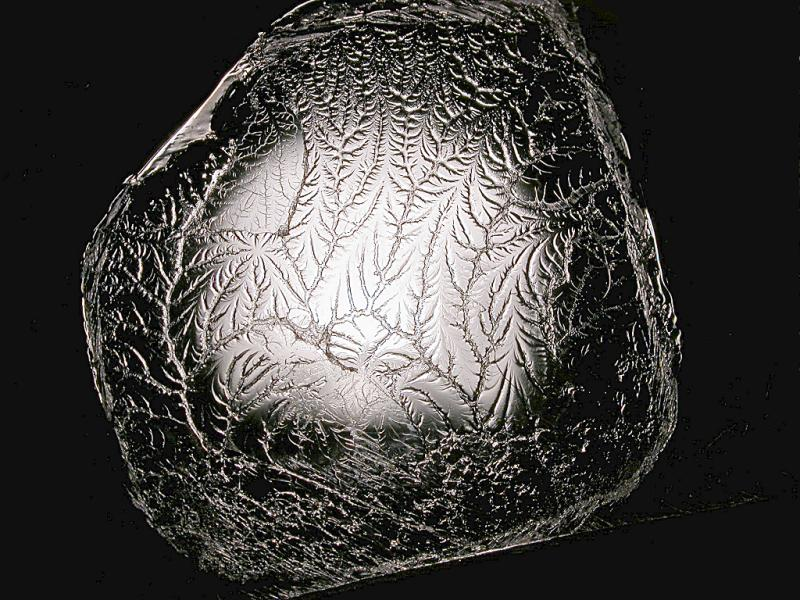
\includegraphics[height=0.9\textheight]{figs/fractal1}
\end{center}
\end{frame}
\begin{frame}
\frametitle{Fractals: high voltage dielectric breakdown}
\framesubtitle{Lichtenberg: Branching discharges decrease to hairlike then to
molecular}
\begin{center}
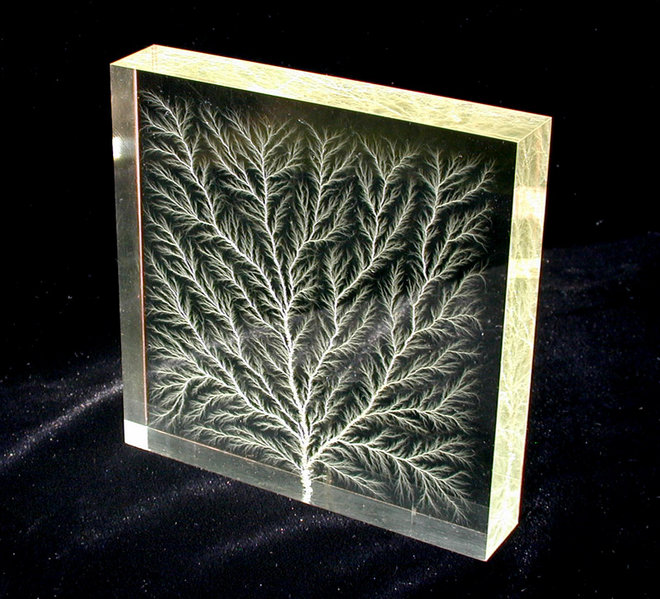
\includegraphics[height=0.9\textheight]{figs/fractal2}
\end{center}
\end{frame}
\begin{frame}
\frametitle{Fractals: Microwaving a CD}
\framesubtitle{Heat vaporizes the aluminum leaving fractal metallic islands}
\begin{center}
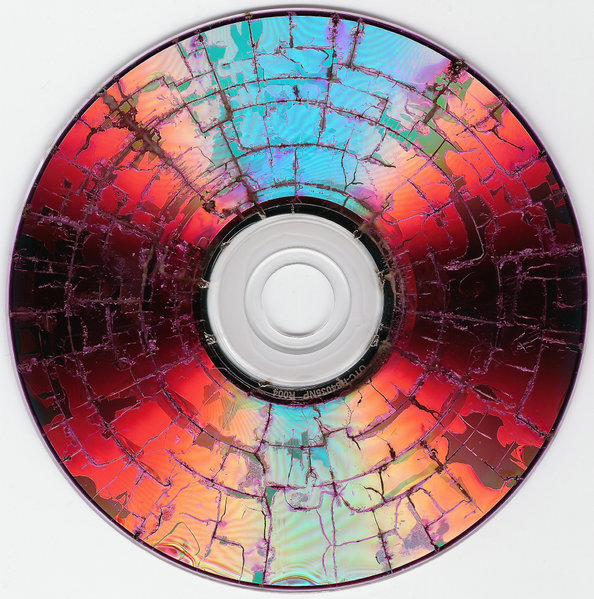
\includegraphics[height=0.9\textheight]{figs/fractal3}
\end{center}
\end{frame}
\begin{frame}
\frametitle{Fractals: Romanesco Broccoli}
\framesubtitle{growth follows fractal pattern}
\begin{center}
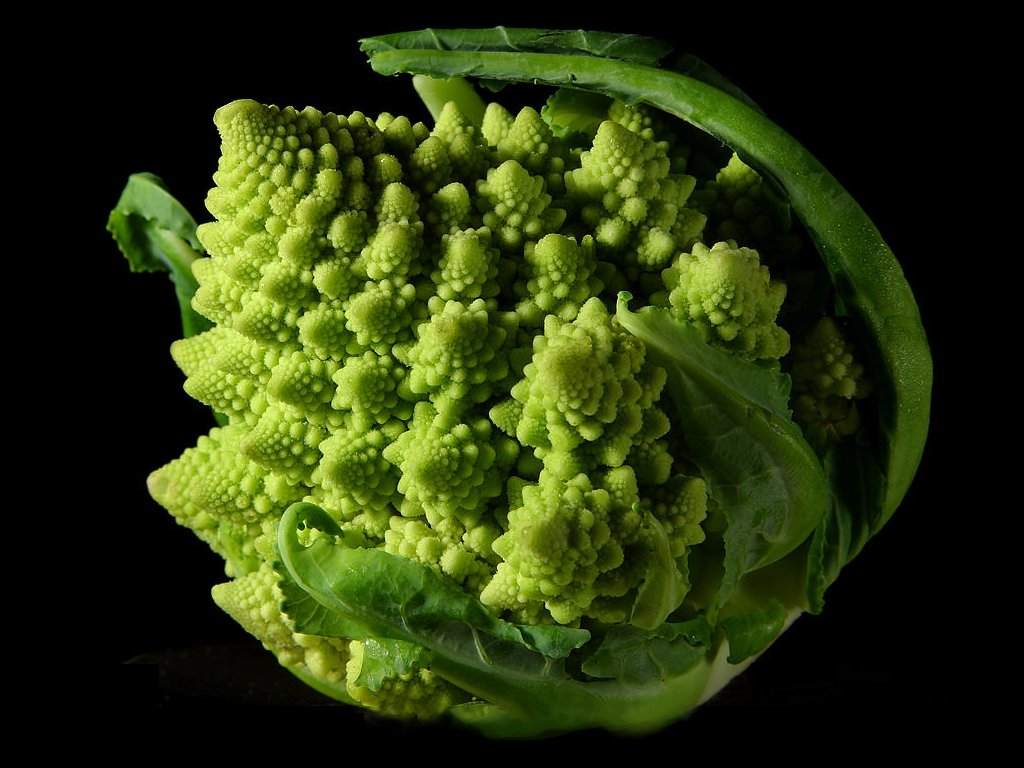
\includegraphics[height=0.9\textheight]{figs/fractal4}
\end{center}
\end{frame}
\begin{frame}
\frametitle{Fractals: Trees}
\framesubtitle{structure follows fractal pattern}
\begin{center}
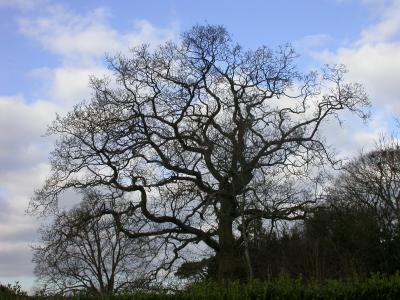
\includegraphics[height=0.9\textheight]{figs/fractal6}
\end{center}
\end{frame}
\begin{frame}
\frametitle{Fractals: Jupiter}
\framesubtitle{Atmosphere modeled with fractals}
\begin{center}
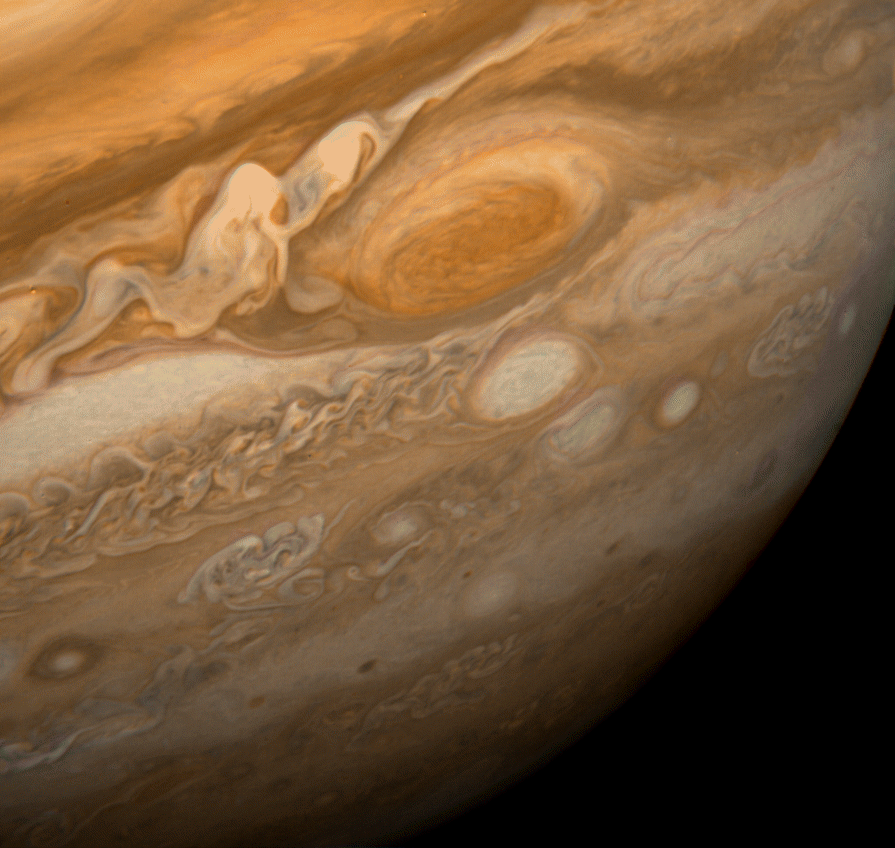
\includegraphics[height=0.9\textheight]{figs/fractal7}
\end{center}
\end{frame}
\begin{frame}
\frametitle{Fractals: Caves}
\framesubtitle{Stalactite/Stalagmite formation}
\begin{center}
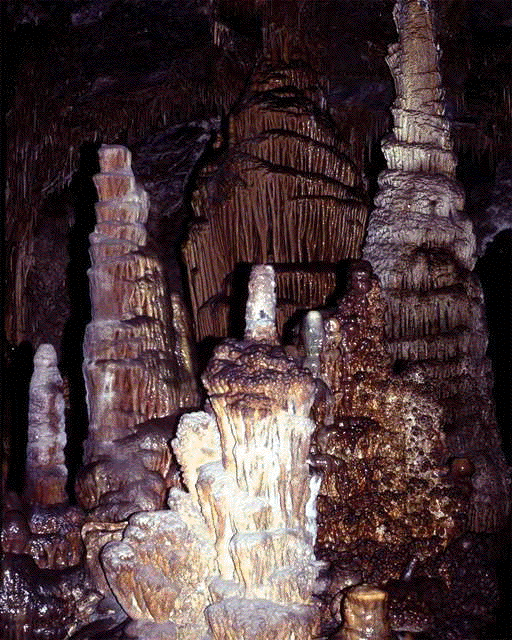
\includegraphics[height=0.9\textheight]{figs/fractal8}
\end{center}
\end{frame}
\begin{frame}
\frametitle{Fractals: Canyons}
\framesubtitle{Erosion patter}
\begin{center}
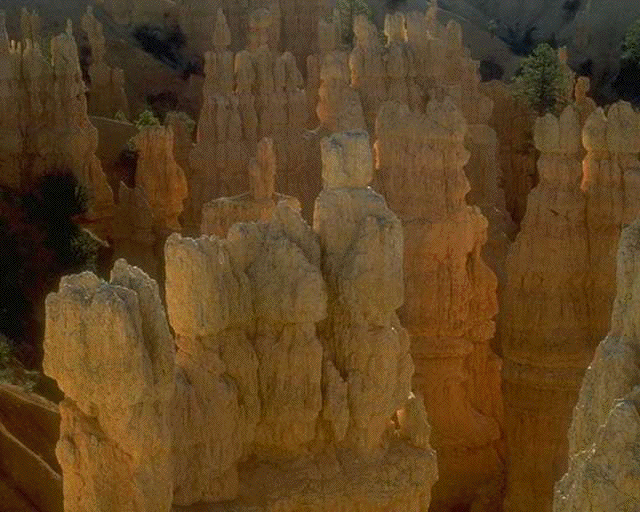
\includegraphics[height=0.9\textheight]{figs/fractal9}
\end{center}
\end{frame}
\begin{frame}
\frametitle{Fractals: Clouds}
\framesubtitle{visualization}
\begin{center}
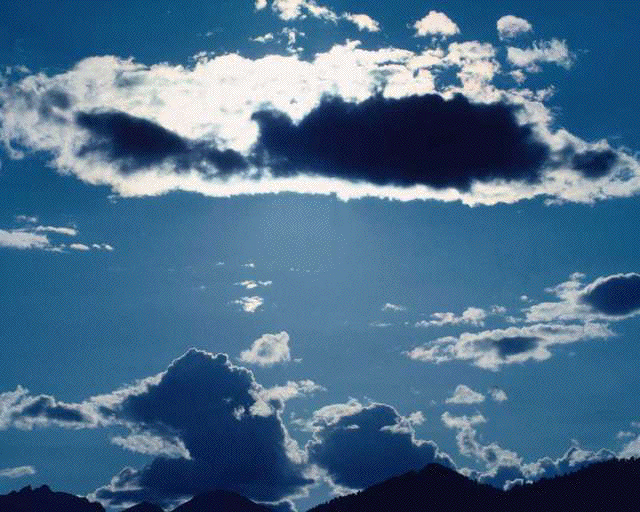
\includegraphics[height=0.9\textheight]{figs/fractal10}
\end{center}
\end{frame}
\begin{frame}
\frametitle{Fractals: Ferns}
\framesubtitle{growth}
\begin{center}
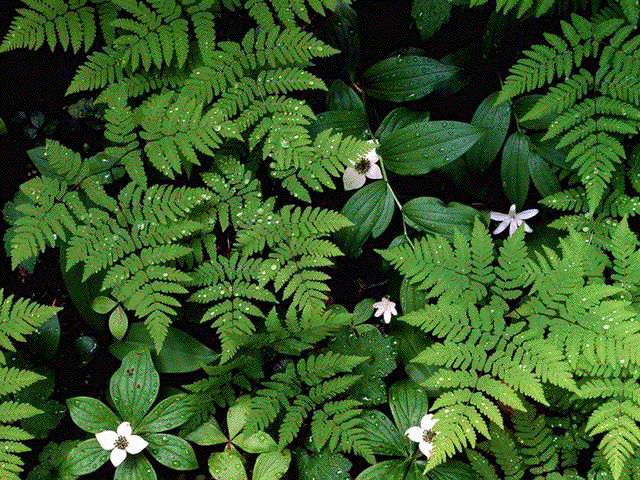
\includegraphics[height=0.9\textheight]{figs/fractal11}
\end{center}
\end{frame}
\begin{frame}
\frametitle{Fractals: Big Trees}
\framesubtitle{growth}
\begin{center}
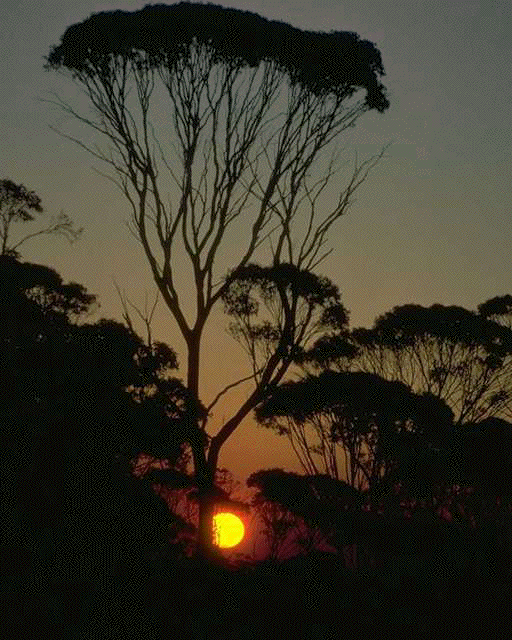
\includegraphics[height=0.9\textheight]{figs/fractal12}
\end{center}
\end{frame}
\begin{frame}
\frametitle{Fractals: leaves}
\framesubtitle{structure}
\begin{center}
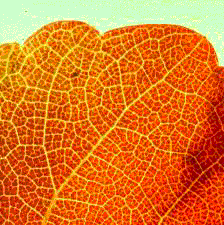
\includegraphics[height=0.9\textheight]{figs/fractal13}
\end{center}
\end{frame}
\begin{frame}
\frametitle{Fractals: lightning}
\framesubtitle{formation}
\begin{center}
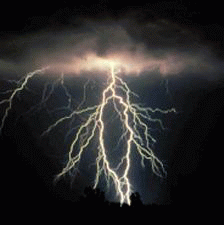
\includegraphics[height=0.9\textheight]{figs/fractal14}
\end{center}
\end{frame}
\begin{frame}
\frametitle{Fractals: cauliflower}
\framesubtitle{structure}
\begin{center}
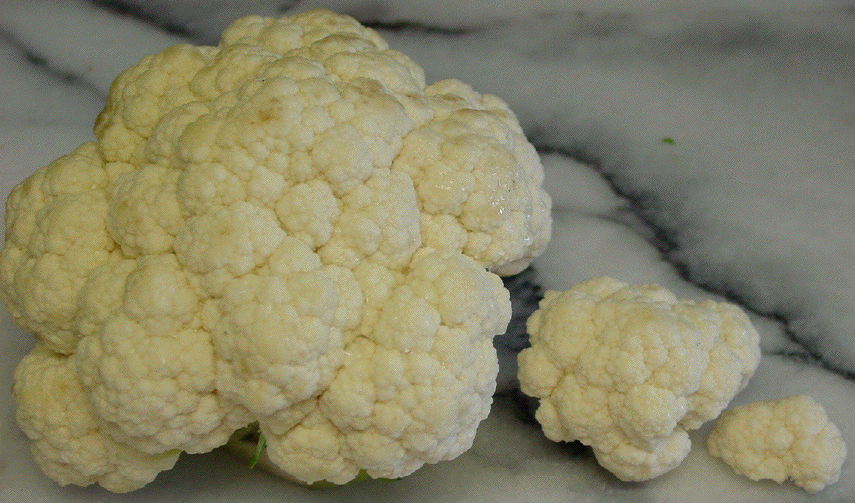
\includegraphics[height=0.9\textheight]{figs/fractal15}
\end{center}
\end{frame}
\begin{frame}
\frametitle{Fractals: mountain}
\framesubtitle{formation}
\begin{center}
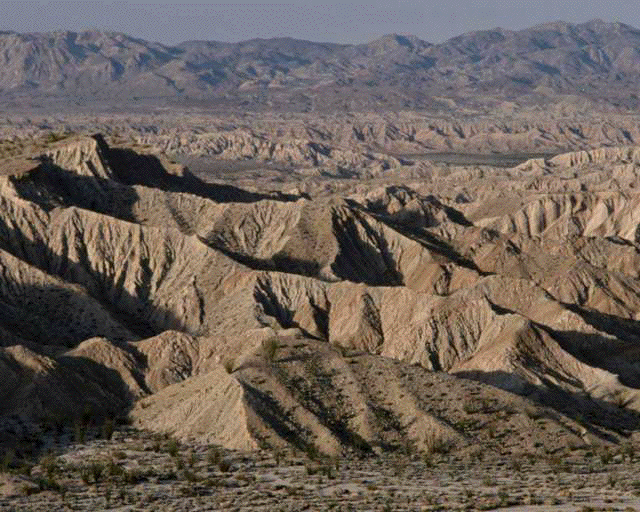
\includegraphics[height=0.9\textheight]{figs/fractal16}
\end{center}
\end{frame}
\begin{frame}
\frametitle{Fractals: mountain}
\framesubtitle{visualization}
\begin{center}
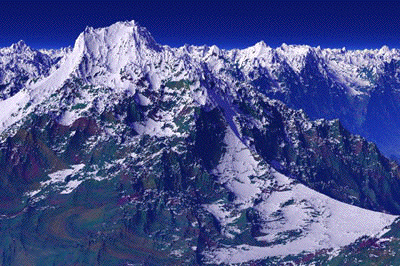
\includegraphics[height=0.9\textheight]{figs/fractal19}
\end{center}
\end{frame}
\begin{frame}
\frametitle{Fractals: Norwegian rivers}
\framesubtitle{structure}
\begin{center}
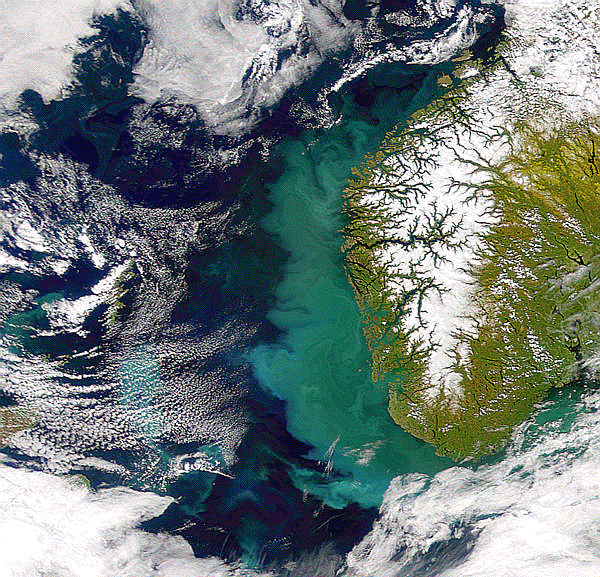
\includegraphics[height=0.9\textheight]{figs/fractal17}
\end{center}
\end{frame}
\begin{frame}
\frametitle{Fractals: waterfalls}
\framesubtitle{pattern}
\begin{center}
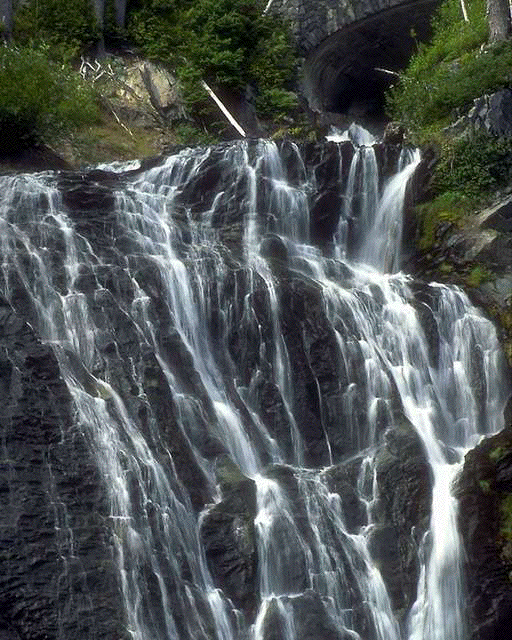
\includegraphics[height=0.9\textheight]{figs/fractal18}
\end{center}
\end{frame}
\begin{frame}
\frametitle{Fractals: coastlines}
\framesubtitle{structure}
\begin{center}
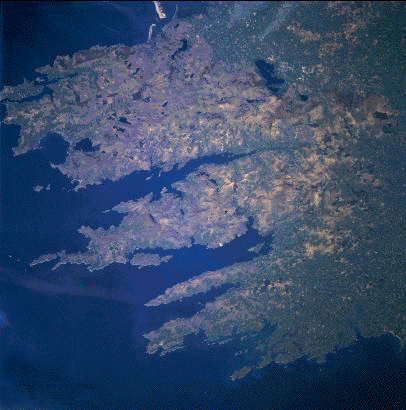
\includegraphics[height=0.9\textheight]{figs/fractal20}
\end{center}
\end{frame}
%%%%%%%%%%%%%%%%%%%%%%%%%%%%%%%%%%%%%%%%%%%%%%%%%%%%%%%%%%%%%%%%%%%%%%%%
\begin{frame}
\frametitle{Fractals: Math}
Recall Complex Numbers: $z \in \mathbb{C}$ means
\begin{equation*}
  z = x + i y,
\end{equation*}
where $i = \sqrt{-1}$
\vspace{0.5cm}

Things to notice:
\begin{itemize}
  \item still think of the $x$-$y$ plane, but now it's in $\mathbb{C}^1$
  instead of $\mathbb{R}^2$
  \item $f(z) = z^2 + 1$ has two roots: $z_{1,2} = \pm i$
  \item $f(z) = z^3 + 1$ has three roots: $z_{1} = 1$, $z_{2,3}=\frac{-1\pm i \sqrt{3}}{2}$
  \item $f(z) = z^4 + 1$ has four roots: $z_{1,2} = \pm1$, $z_{3,4}=\pm i$
\end{itemize}
\end{frame}
%%%%%%%%%%%%%%%%%%%%%%%%%%%%%%%%%%%%%%%%%%%%%%%%%%%%%%%%%%%%%%%%%%%%%%%%
%%%%%%%%%%%%%%%%%%%%%%%%%%%%%%%%%%%%%%%%%%%%%%%%%%%%%%%%%%%%%%%%%%%%%%%%
\begin{frame}
\frametitle{Fractals: Newton's Algorithm}
The big idea:
\begin{itemize}
  \item Take a complex function like $f(z) = z^3 + 1$
  \item Pick a bunch of initial guesses $Z_0$ as the roots
  \item Run Newton's Method
  \item The initial guesses $Z_0$ will each converge to one of $n=3$ roots
  \item Color each guess in the plane depending on the root to which it converged
\end{itemize}
\begin{center}
  \pgfimage[height=4cm]{figs/fractal_newton}
\end{center}
\end{frame}
%%%%%%%%%%%%%%%%%%%%%%%%%%%%%%%%%%%%%%%%%%%%%%%%%%%%%%%%%%%%%%%%%%%%%%%%
%%%%%%%%%%%%%%%%%%%%%%%%%%%%%%%%%%%%%%%%%%%%%%%%%%%%%%%%%%%%%%%%%%%%%%%%
\begin{frame}
\frametitle{Secant Method}

\vspace{4ex}
\begin{center}
	\pgfimage[height=3cm]{./figs/secant}
\end{center}

Given two guesses $x_{k-1}$ and $x_k$, the next guess at the root
is where the line through $f(x_{k-1})$ and $f(x_k)$
crosses the $x$ axis.



% ------------
\end{frame}
%%%%%%%%%%%%%%%%%%%%%%%%%%%%%%%%%%%%%%%%%%%%%%%%%%%%%%%%%%%%%%%%%%%%%%%%
%%%%%%%%%%%%%%%%%%%%%%%%%%%%%%%%%%%%%%%%%%%%%%%%%%%%%%%%%%%%%%%%%%%%%%%%
\begin{frame}
\frametitle{Secant Method}

Given
\begin{align*}
    x_k     &= \mathrm{current\ guess\ at\ the\ root}\\
    x_{k-1} &= \mathrm{previous\ guess\ at\ the\ root}
\end{align*}

Approximate the first derivative with
\begin{equation*}
    f'(x_k) \approx \frac{f(x_k) - f(x_{k-1})}{x_k - x_{k-1}}
\end{equation*}

Substitute approximate $f'(x_k)$ into formula for Newton's method
\begin{equation*}
    x_{k+1} = x_k - \frac{f(x_k)}{f'(x_k)}
\end{equation*}
to get
\begin{equation*}
    x_{k+1} = x_k - f(x_k) \left[ \frac{x_k - x_{k-1}}{f(x_k) - f(x_{k-1})} \right]
\end{equation*}



% ------------
\end{frame}
%%%%%%%%%%%%%%%%%%%%%%%%%%%%%%%%%%%%%%%%%%%%%%%%%%%%%%%%%%%%%%%%%%%%%%%%
%%%%%%%%%%%%%%%%%%%%%%%%%%%%%%%%%%%%%%%%%%%%%%%%%%%%%%%%%%%%%%%%%%%%%%%%
\begin{frame}
\frametitle{Secant Method}

\vspace{3ex}
Two versions of this formula are (equivalent in exact math)
\begin{equation*}
    x_{k+1} = x_k - f(x_k) \left[ \frac{x_k - x_{k-1}}{f(x_k) - f(x_{k-1})} \right]  \tag{$\star$}
\end{equation*}
and
\begin{equation*}
    x_{k+1} = \frac{f(x_k) x_{k-1} - f(x_{k-1}) x_k}{f(x_k) - f(x_{k-1})}  \tag{$\star\star$}
\end{equation*}

Equation~($\star$) is better since it is of the form $x_{k+1} = x_k + \Delta$.
Even if $\Delta$ is inaccurate the change in the estimate of the
root will be small at convergence because $f(x_k)$ will also
be small.

Equation~($\star\star$) is susceptible to catastrophic cancellation:
\vspace{0.0cm}
\begin{itemize}
    \item   $f(x_k)\rightarrow f(x_{k-1})$ as convergence approaches,
            so cancellation error in denominator can be large.
    \item   $|f(x)|\rightarrow 0$ as convergence approaches,
            so underflow is possible
\end{itemize}



% ------------
\end{frame}
%%%%%%%%%%%%%%%%%%%%%%%%%%%%%%%%%%%%%%%%%%%%%%%%%%%%%%%%%%%%%%%%%%%%%%%%
%%%%%%%%%%%%%%%%%%%%%%%%%%%%%%%%%%%%%%%%%%%%%%%%%%%%%%%%%%%%%%%%%%%%%%%%
\begin{frame}[fragile]
\frametitle{Secant Algorithm}

\begin{lstlisting}[mathescape,caption=,label=algo:secant]
  initialize:  $x_1 = \ldots$, $x_2 = \ldots$                   
  for $k=2,3\ldots$                                           
    $x_{k+1} = x_k - f(x_k) (x_k - x_{k-1})/(f(x_k) - f(x_{k-1}) )$  
    if converged, stop       
  end
\end{lstlisting}





% ------------
\end{frame}
%%%%%%%%%%%%%%%%%%%%%%%%%%%%%%%%%%%%%%%%%%%%%%%%%%%%%%%%%%%%%%%%%%%%%%%%
%%%%%%%%%%%%%%%%%%%%%%%%%%%%%%%%%%%%%%%%%%%%%%%%%%%%%%%%%%%%%%%%%%%%%%%%
\begin{frame}
\frametitle{Secant Example}

Solve:
\begin{equation*}
    x - x^{1/3} - 2 = 0
\end{equation*}

\vspace{2ex}
\begin{center}
  \small
    \begin{tabular}{cccc}
       $k$ &   $x_{k-1}$  &    $x_k$   & $f(x_k)$                  \\ \hline
        0  &  4           & 3          & $-0.44224957$               \\
        1  &  3           & 3.51734262 & $-0.00345547$               \\
        2  &  3.51734262  & 3.52141665 & $0.00003163 $              \\
        3  &  3.52141665  & 3.52137970 & $-2.034\times 10^{-9}$  \\
        4  &  3.52137959  & 3.52137971 & $-1.332\times 10^{-15}$ \\
        5  &  3.52137971  & 3.52137971 &  0.0                      \\
        \end{tabular}
\end{center}

\vspace{4ex}

\textbf{Conclusions:}
\vspace{0.0cm}
\begin{itemize}
    \item   Converges almost as quickly as Newton's method ($r\approx
1.62$).
    \item   There is no need to compute $f'(x)$.
    \item   The algorithm is simple.
    \item   Two initial guesses are necessary
    \item   Iterations are not guaranteed to stay inside an ordinal bracket.
\end{itemize}




% ------------
\end{frame}
%%%%%%%%%%%%%%%%%%%%%%%%%%%%%%%%%%%%%%%%%%%%%%%%%%%%%%%%%%%%%%%%%%%%%%%%
%%%%%%%%%%%%%%%%%%%%%%%%%%%%%%%%%%%%%%%%%%%%%%%%%%%%%%%%%%%%%%%%%%%%%%%%
\begin{frame}
\frametitle{Divergence of Secant Method}

\vspace{4ex}
\begin{center}
	\pgfimage[height=3cm]{./figs/secantFails}
%%     \ifthenelse{\equal{\OS}{Mac}}
%%         {\epsfig{file=:eps:secantFails.eps,scale=0.9}}
%%         {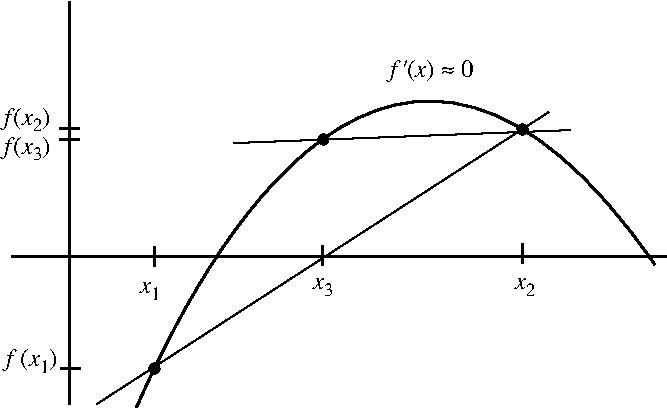
\epsfig{file=eps/secantFails.eps,scale=0.9}}
\end{center}

\vspace{2ex}
Since
\begin{equation*}
    x_{k+1} = x_k - f(x_k) \left[ \frac{x_k - x_{k-1}}{f(x_k) - f(x_{k-1})} \right]
\end{equation*}

the new guess, $x_{k+1}$, will be far from the old guess
whenever $f(x_k)\approx f(x_{k-1})$ and $|f(x)|$ is not small.


% ------------
\end{frame}
%%%%%%%%%%%%%%%%%%%%%%%%%%%%%%%%%%%%%%%%%%%%%%%%%%%%%%%%%%%%%%%%%%%%%%%%
%%%%%%%%%%%%%%%%%%%%%%%%%%%%%%%%%%%%%%%%%%%%%%%%%%%%%%%%%%%%%%%%%%%%%%%%
\begin{frame}
\frametitle{Summary}

\begin{itemize}
\item   Plot $f(x)$ before searching for roots
		\vspace{2ex}
\item   Bracketing finds coarse interval containing roots
		and singularities
		\vspace{2ex}
\item   Bisection is robust, but converges slowly
		\vspace{2ex}
\item   Newton's Method
	\begin{itemize}
		\item   Requires $f(x)$ and $f'(x)$.
		\item   Iterates are not confined to initial bracket.
		\item   Converges rapidly ($r=2$).
		\item   Diverges if $f'(x)\approx 0$ is encountered.
	\end{itemize}
		\vspace{2ex}
\item   Secant Method
	\begin{itemize}
		\item   Uses $f(x)$ values to approximate $f'(x)$.
		\item   Iterates are not confined to initial bracket.
		\item   Converges almost as rapidly as Newton's method ($r\approx
1.62)$.
		\item   Diverges if $f'(x)\approx 0$ is encountered.
	\end{itemize}
\end{itemize}




% ------------
\end{frame}
%%%%%%%%%%%%%%%%%%%%%%%%%%%%%%%%%%%%%%%%%%%%%%%%%%%%%%%%%%%%%%%%%%%%%%%%
\begin{frame}[fragile]
\frametitle{\texttt{fzero} Function}

\texttt{fzero} is a hybrid method that combines bisection,
secant and reverse quadratic interpolation

\vspace{3ex}
\begin{lstlisting}[language=matlab]
r = fzero('fun',x0)
r = fzero('fun',x0,options)
r = fzero('fun',x0,options,arg1,rg2,...)
\end{lstlisting}

\vspace{3ex}
\texttt{x0} can be a scalar or a two element vector
\begin{itemize}
    \item   If \texttt{x0} is a scalar, \texttt{fzero} tries to
            create its own bracket.
    \item   If \texttt{x0} is a two element vector, \texttt{fzero}
            uses the vector as a bracket.
\end{itemize}



% ------------
\end{frame}
%%%%%%%%%%%%%%%%%%%%%%%%%%%%%%%%%%%%%%%%%%%%%%%%%%%%%%%%%%%%%%%%%%%%%%%%
%%%%%%%%%%%%%%%%%%%%%%%%%%%%%%%%%%%%%%%%%%%%%%%%%%%%%%%%%%%%%%%%%%%%%%%%
\begin{frame}
\frametitle{Reverse Quadratic Interpolation}

\vspace{2ex}
Find the point where the $x$ axis intersects the sideways parabola passing
through three pairs of $(x,f(x))$ values.

\begin{center}
	\pgfimage[height=5cm]{./figs/fzeroPicture}
\end{center}

% ------------
\end{frame}
%%%%%%%%%%%%%%%%%%%%%%%%%%%%%%%%%%%%%%%%%%%%%%%%%%%%%%%%%%%%%%%%%%%%%%%%
%%%%%%%%%%%%%%%%%%%%%%%%%%%%%%%%%%%%%%%%%%%%%%%%%%%%%%%%%%%%%%%%%%%%%%%%
\begin{frame}
\frametitle{\texttt{fzero} Function}

\texttt{fzero} chooses next root as
\begin{itemize}
    \item   Result of reverse quadratic interpolation (RQI) if that result
            is inside the current bracket.
    \item   Result of secant step if RQI fails, and if the result of secant
            method is in inside the current bracket.
    \item   Result of bisection step if both RQI and secant method fail
            to produce guesses inside the current bracket.
\end{itemize}

% ------------
\end{frame}
%%%%%%%%%%%%%%%%%%%%%%%%%%%%%%%%%%%%%%%%%%%%%%%%%%%%%%%%%%%%%%%%%%%%%%%%
%%%%%%%%%%%%%%%%%%%%%%%%%%%%%%%%%%%%%%%%%%%%%%%%%%%%%%%%%%%%%%%%%%%%%%%%
\begin{frame}[fragile]
\frametitle{\texttt{fzero} Function}

Optional parameters to control \texttt{fzero} are specified with
the \texttt{optimset} function.

\bigskip
Tell \texttt{fzero} to display the results of each step:
\vspace{0.0cm}
\begin{lstlisting}[language=matlab]
>> options = optimset('Display','iter');
>> x = fzero('myFun',x0,options)
\end{lstlisting}

\vspace{3ex}

Tell \texttt{fzero} to use a relative tolerance of $5\times10^{-9}$:
\vspace{0.0cm}
\begin{lstlisting}[language=matlab]
>> options = optimset('TolX',5e-9);
>> x = fzero('myFun',x0,options)
\end{lstlisting}

\vspace{3ex}

Tell \texttt{fzero} to suppress all printed output, and
use a relative tolerance of $5\times10^{-4}$:
\vspace{0.0cm}
\begin{lstlisting}[language=matlab]
>> options = optimset('Display','off','TolX',5e-4);
>> x = fzero('myFun',x0,options)
\end{lstlisting}

% ------------
\end{frame}
%%%%%%%%%%%%%%%%%%%%%%%%%%%%%%%%%%%%%%%%%%%%%%%%%%%%%%%%%%%%%%%%%%%%%%%%
%%%%%%%%%%%%%%%%%%%%%%%%%%%%%%%%%%%%%%%%%%%%%%%%%%%%%%%%%%%%%%%%%%%%%%%%
\begin{frame}[fragile]
\frametitle{\texttt{fzero} Function}

Allowable options (specified via \texttt{optimset}):
\begin{center}
    \renewcommand{\arraystretch}{1.3}
    \small
    \begin{tabular}{llp{12cm}}
        \multicolumn{1}{c}{Option type}
        & \multicolumn{1}{c}{Value}
        & \multicolumn{1}{c}{Effect}  \\
        \hline
        \texttt{'Display'} & \texttt{'iter'}  & Show results of each iteration \\
                           & \texttt{'final'} & Show root and original bracket \\
                           & \texttt{'off'}   & Suppress all print out \\[16pt]
        \texttt{'TolX'}    & \texttt{tol}     & Iterate until\\
                           &                  & \qquad$\displaystyle\left|\Delta x\right|<\max\left[\mathtt{tol},\mathtt{tol}*\mathtt{a}, \mathtt{tol}*\mathtt{b}\right]$\\
                           &                  & where $\Delta x = (b-a)/2$, and $[a,b]$ is the current bracket. \\
         \hline
    \end{tabular}
\end{center}

\vspace{2ex}
The default values of \texttt{'Display'} and \texttt{'TolX'}
are equivalent to
\begin{lstlisting}[language=matlab]
options = optimset('Display','iter','TolX',eps)
\end{lstlisting}

% ------------
\end{frame}
%%%%%%%%%%%%%%%%%%%%%%%%%%%%%%%%%%%%%%%%%%%%%%%%%%%%%%%%%%%%%%%%%%%%%%%%
\begin{frame}[fragile]
\frametitle{\texttt{fzero} example}
Take
\begin{equation*}
  f(x) = x^{10} - 1
\end{equation*}

\vspace{1cm}
\begin{lstlisting}[language=matlab]
>> f = @(x)x.^10 - 1;
>>  options = optimset('display','iter');
>> [x,fx]=fzero(f,0.5,options)
\end{lstlisting}
\end{frame}

\end{document}
